\section{Calculus and Parametric Equations}\label{sec:par_calc}

The previous section defined curves based on parametric equations. In this section we'll employ the techniques of calculus to study these curves.

We are still interested in lines tangent to points on a curve. They describe how the $y$-values are changing with respect to the $x$-values, they are useful in making approximations, and they indicate instantaneous direction of travel.

The slope of the tangent line is still $\frac{dy}{dx}$, and the Chain Rule allows us to calculate this in the context of parametric equations. If $x=f(t)$ and $y=g(t)$, the Chain Rule states that $$\frac{dy}{dt} = \frac{dy}{dx}\cdot\frac{dx}{dt}.$$
Solving for $\frac{dy}{dx}$, we get 
$$\frac{dy}{dx} = \frac{dy}{dt}\Bigg/\frac{dx}{dt} = \frac{g\primeskip'(t)}{\fp(t)},$$
provided that $\fp(t)\neq 0$. This is important so we label it a Key Idea.

\keyidea{idea:dydxpar}{Finding $\frac{dy}{dx}$ with Parametric Equations.}
{Let $x=f(t)$ and $y=g(t)$, where $f$ and $g$ are differentiable on some open interval $I$ and $\fp(t)\neq 0$ on $I$. Then \index{parametric equations!finding $\frac{dy}{dx}$}\index{derivative!parametric equations}
$$\frac{dy}{dx} = \frac{g\primeskip'(t)}{\fp(t)}.$$
}

We use this to define the tangent line.

\definition{def:tangent_par}{Tangent and Normal Lines}
{Let a curve $C$ be parametrized by $x=f(t)$ and $y=g(t)$, where $f$ and $g$ are differentiable functions on some interval $I$ containing $t=t_0$. The \textbf{tangent line} to $C$ at $t=t_0$ is the line through $\big(f(t_0),g(t_0)\big)$ with slope $m=g\primeskip'(t_0)/\fp(t_0)$, provided $\fp(t_0)\neq 0$.\\

The \textbf{normal line} to $C$ at $t=t_0$ is the line through $\big(f(t_0),g(t_0)\big)$ with slope $m=-\fp(t_0)/g\primeskip'(t_0)$, provided $g\primeskip'(t_0)\neq 0$.\index{tangent line}\index{normal line}\index{parametric equations!tangent line}\index{parametric equations!normal line}
}

The definition leaves two special cases to consider. When the tangent line is horizontal, the normal line is undefined by the above definition as $g\primeskip'(t_0)=0$. Likewise, when the normal line is horizontal, the tangent line is undefined. It seems reasonable that these lines be defined (one can draw a line tangent to the ``right side'' of a circle, for instance), so we add the following to the above definition.

	
\begin{enumerate}
	\item If the tangent line at $t=t_0$ has a slope of 0, the normal line to $C$ at $t=t_0$ is the line $x=f(t_0)$.
	\item		If the normal line at $t=t_0$ has a slope of 0, the tangent line to $C$ at $t=t_0$ is the line $x=f(t_0)$.
	\end{enumerate}
	
\example{ex_parcalc1}{Tangent and Normal Lines to Curves}{
Let $x=5t^2-6t+4$ and $y=t^2+6t-1$, and let $C$ be the curve defined by these equations.
\begin{enumerate}
	\item Find the equations of the tangent and normal lines to $C$ at $t=3$.
	\item	Find where $C$ has vertical and horizontal tangent lines.
\end{enumerate}
	}
	{\begin{enumerate}
		\item We start by computing $\fp(t) = 10t-6$ and $g\primeskip'(t) =2t+6$. Thus $$\frac{dy}{dx} = \frac{2t+6}{10t-6}.$$
		Make note of something that might seem unusual: $\frac{dy}{dx}$ is a function of $t$, not $x$. Just as points on the curve are found in terms of $t$, so are the slopes of the tangent lines.
		
		The point on $C$ at $t=3$ is $(31,26)$. The slope of the tangent line is $m=1/2$ and the slope of the normal line is $m=-2$. Thus,
		\begin{itemize}
			\item the equation of the tangent line is $\ds y=\frac12(x-31)+26$, and
			\item	the equation of the normal line is $\ds y=-2(x-31)+26$.
		\end{itemize}
		This is illustrated in Figure \ref{fig:parcalc1}.
		\mfigure{.5}{Graphing tangent and normal lines in Example \ref{ex_parcalc1}.}{fig:parcalc1}{figures/figparcalc1}
		
		\item		To find where $C$ has a horizontal tangent line, we set $\frac{dy}{dx}=0$ and solve for $t$. In this case, this amounts to setting $g\primeskip'(t)=0$ and solving for $t$ (and making sure that $\fp(t)\neq 0$). 
		$$g\primeskip'(t)=0 \quad \Rightarrow \quad 2t+6=0 \quad \Rightarrow \quad t=-3.$$
		The point on $C$ corresponding to $t=-3$ is $(67,-10)$; the tangent line at that point is horizontal (hence with equation $y=-10$).
		
		To find where $C$ has a vertical tangent line, we find where it has a horizontal normal line, and set $-\frac{\fp(t)}{g\primeskip'(t)}=0$. This amounts to setting $\fp(t)=0$ and solving for $t$ (and making sure that $g\primeskip'(t)\neq 0$). 
		$$\fp(t)=0 \quad \Rightarrow \quad 10t-6=0 \quad \Rightarrow \quad t=0.6.$$
		The point on $C$ corresponding to $t=0.6$ is $(2.2,2.96)$. The tangent line at that point is $x=2.2$.
	
		The points where the tangent lines are vertical and horizontal are indicated on the graph in Figure \ref{fig:parcalc1}.
		\end{enumerate}
		\vskip-\baselineskip
	}\\
	
	\example{ex_parcalc2}{Tangent and Normal Lines to a Circle}{
	\begin{enumerate}
		\item Find where the unit circle, defined by $x=\cos t$ and $y=\sin t$ on $[0,2\pi]$, has vertical and horizontal tangent lines. 
		\item	 Find the equation of the normal line at $t=t_0$.
		\end{enumerate}
		}
		{\begin{enumerate}
			\item We compute the derivative following Key Idea \ref{idea:dydxpar}:
			$$\frac{dy}{dx} = \frac{g\primeskip'(t)}{\fp(t)} = -\frac{\cos t}{\sin t}.$$
			The derivative is $0$ when $\cos t= 0$; that is, when $t=\pi/2,\ 3\pi/2$. These are the points $(0,1)$ and $(0,-1)$ on the circle.
			
			The normal line is horizontal (and hence, the tangent line is vertical) when $\sin t=0$; that is, when $t= 0,\ \pi,\ 2\pi$, corresponding to the points $(-1,0)$ and $(0,1)$ on the circle. These results should make intuitive sense.
			\item		The slope of the normal line at $t=t_0$ is $\ds m=\frac{\sin t_0}{\cos t_0} = \tan t_0$. This normal line goes through the point $(\cos t_0,\sin t_0)$, giving the line \begin{align*}y &=\frac{\sin t_0}{\cos t_0}(x-\cos t_0) + \sin t_0\\	
							&= (\tan t_0)x,
\end{align*}
as long as $\cos t_0\neq 0$. It is an important fact to recognize that the normal lines to a circle pass through its center, as illustrated in Figure \ref{fig:parcalc2}. Stated in another way, any line that passes through the center of a circle intersects the circle at right angles.
\mfigure{.4}{Illustrating how a circle's normal lines pass through its center.}{fig:parcalc2}{figures/figparcalc2}
		\end{enumerate}
	\vskip-1.5\baselineskip
		}\\

\clearpage

\example{ex_parcalc3}{Tangent lines when $\frac{dy}{dx}$ is not defined}
{Find the equation of the tangent line to the astroid $x=\cos^3 t$, $y=\sin^3t$ at $t=0$, shown in Figure \ref{fig:parcalc3}.
}
{We start by finding $x\primeskip'(t)$ and $y\primeskip'(t)$:
$$ x\primeskip'(t) = -3\sin t\cos^2t, \qquad y\primeskip'(t) = 3\cos t\sin^2t.$$
Note that both of these are 0 at $t=0$; the curve is not smooth at $t=0$ forming a cusp on the graph. Evaluating $\frac{dy}{dx}$ at this point returns the indeterminate form of ``0/0''. 
%$\frac{dy}{dx}$:
%$$\frac{dy}{dx} = \frac{-3\sin t\cos^2t}{3\cos t\sin^2t} = -\frac{\sin t}{\cos t},$$ as long as $\cos t\neq 0$ and $\sin t\neq 0$. When $t=0$, it is tempting to declare that $$\frac{dy}{dx} = -\frac{\sin 0}{\cos 0} = 0,$$ but this overlooks the fact that we canceled earlier with the stipulation that $\sin t\neq 0$. In fact, the graph of the curve has a cusp at $t=0$, as both $x\primeskip'=0$ and $y\primeskip'=0$. 

We can, however, examine the slopes of tangent lines near $t=0$, and take the limit as $t\to 0$. 
\begin{align*}
\lim_{t\to0} \frac{y\primeskip'(t)}{x\primeskip'(t)} &=\lim_{t\to0} \frac{3\cos t\sin^2t}{-3\sin t\cos^2t} \quad \text{\small (We can cancel as $t\neq 0$.)}\\
					&= \lim_{t\to0} -\frac{\sin t}{\cos t}\\
					&= 0.
\end{align*}
We have accomplished something significant. When the derivative $\frac{dy}{dx}$ returns an indeterminate form at $t=t_0$, we can define its value by setting it to be $\ds \lim_{t\to t_0} $$\frac{dy}{dx}$, if that limit exists. This allows us to find slopes of tangent lines at cusps, which can be very beneficial. 
\mfigure{.8}{A graph of an astroid.}{fig:parcalc3}{figures/figplanecurve1}

We found the slope of the tangent line at $t=0$ to be 0; therefore the tangent line is $y=0$, the $x$-axis. 
}\\

\noindent\textbf{\large Concavity}\\

We continue to analyze curves in the plane by considering their concavity; that is, we are interested in $\frac{d^2y}{dx^2}$, ``the second derivative of $y$ with respect to $x$.'' To find this, we need to find the derivative of $\frac{dy}{dx}$ with respect to $x$; that is,  $$\frac{d^2y}{dx^2}=\frac{d}{dx}\left[\frac{dy}{dx}\right],$$ but recall that $\frac{dy}{dx}$ is a function of $t$, not $x$, making this computation not straightforward. \index{concavity}\index{parametric equations!concavity}

To make the upcoming notation a bit simpler, let $h(t) = \frac{dy}{dx}$. We want $\frac{d}{dx}[h(t)]$; that is, we want $\frac{dh}{dx}$. We again appeal to the Chain Rule. Note:
$$\frac{dh}{dt} = \frac{dh}{dx}\cdot\frac{dx}{dt} \quad \Rightarrow \quad \frac{dh}{dx} = \frac{dh}{dt}\Bigg/\frac{dx}{dt}.$$

In words, to find $\frac{d^2y}{dx^2}$, we first take the derivative of $\frac{dy}{dx}$ \textit{with respect to $t$}, then divide by $x\primeskip'(t)$. We restate this as a Key Idea.

\keyidea{idea:second_der_par}{Finding $\frac{d^2y}{dx^2}$ with Parametric Equations}
{Let $x=f(t)$ and $y=g(t)$ be twice differentiable functions on an open interval $I$, where $\fp(t)\neq 0$ on $I$. Then 
\index{parametric equations!finding $\frac{d^2y}{dx^2}$}
$$\frac{d^2y}{dx^2}\quad = \quad\frac{d}{dt}\left[\frac{dy}{dx}\right]\Bigg/\frac{dx}{dt} \quad=\quad \frac{d}{dt}\left[\frac{dy}{dx}\right]\Bigg/\fp(t).$$ 
}

Examples will help us understand this Key Idea.\\

\example{ex_parcalc4}{Concavity of Plane Curves}{
Let $x=5t^2-6t+4$ and $y=t^2+6t-1$ as in Example \ref{ex_parcalc1}. Determine the $t$-intervals on which the graph is concave up/down.}
{Concavity is determined by the second derivative of $y$ with respect to $x$, $\frac{d^2y}{dx^2}$, so we compute that here following Key Idea \ref{idea:second_der_par}.

In Example \ref{ex_parcalc1}, we found $\ds\frac{dy}{dx} = \frac{2t+6}{10t-6}$ and $\fp(t) = 10t-6$. So:
\begin{align*}
\frac{d^2y}{dx^2} &= \frac{d}{dt}\left[\frac{2t+6}{10t-6}\right]\Bigg/(10t-6) \\
				&= -\frac{72}{(10t-6)^2}\Bigg/(10t-6)\\
				&= -\frac{72}{(10t-6)^3} \\&= -\frac{9}{(5t-3)^3}
\end{align*}
\mfigure{.5}{Graphing the parametric equations in Example \ref{ex_parcalc4} to demonstrate concavity.}{fig:parcalc4}{figures/figparcalc4}

The graph of the parametric functions is concave up when $\frac{d^2y}{dx^2} > 0$ and concave down when $\frac{d^2y}{dx^2} <0$. We determine the intervals when the second derivative is greater/less than 0 by first finding when it is 0 or undefined.

As the numerator of $\ds -\frac{9}{(5t-3)^3}$ is never 0, $\frac{d^2y}{dx^2} \neq 0$ for all $t$. It is undefined when $5t-3=0$; that is, when $t= 3/5$. Following the work established in Section \ref{sec:concavity}, we look at values of $t$ greater/less than $3/5$ on a number line:

\begin{center}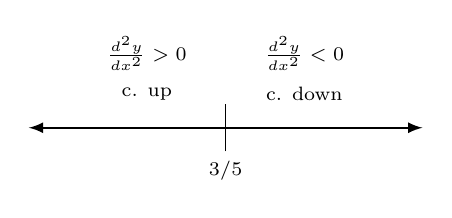
\begin{tikzpicture}[>=latex]
		\draw [<->, thick] (-2.5,0) -- (2.5,0);
		\foreach \x / \y  in %
					{0/{$3/5$}}
		{\draw (\x,-.3) node[below] {\scriptsize \parbox{40pt}{\centering \y}} -- (\x,.3);}
		\draw (-1,.75) node {\scriptsize \parbox{50pt}{\centering $\ds \frac{d^2y}{dx^2}>0$ \\[5pt] c. up }};
		\draw (1,.75) node {\scriptsize \parbox{50pt}{\centering $\ds\frac{d^2y}{dx^2}<0$ \\[5pt] c. down }};
\end{tikzpicture}\end{center}

Reviewing Example \ref{ex_parcalc1}, we see that when $t=3/5=0.6$, the graph of the parametric equations has a vertical tangent line. This point is also a point of inflection for the graph, illustrated in Figure \ref{fig:parcalc4}.
}\\

\example{ex_parcalc5}{Concavity of Plane Curves}{
Find the points of inflection of the graph of the parametric equations $x=\sqrt{t}$, $y=\sin t$, for $0\leq t\leq 16$.}
{We need to compute $\frac{dy}{dx}$ and $\frac{d^2y}{dx^2}$. 
$$\frac{dy}{dx} = \frac{y\primeskip'(t)}{x\primeskip'(t)} = \frac{\cos t}{1/(2\sqrt{t})} = 2\sqrt{t}\cos t.$$
$$\frac{d^2y}{dx^2} = \frac{\frac{d}{dt}\left[\frac{dy}{dx}\right]}{x\primeskip'(t)} = \frac{\cos t/\sqrt{t}-2\sqrt{t}\sin t}{1/(2\sqrt{t})}=2\cos t-4t\sin t.$$
The points of inflection are found by setting $\frac{d^2y}{dx^2}=0$. This is not trivial, as equations that mix polynomials and trigonometric functions generally do not have ``nice'' solutions. 

In Figure \ref{fig:parcalc5}(a) we see a plot of the second derivative. It shows that it has zeros at approximately $t=0.5,\ 3.5,\ 6.5,\ 9.5,\ 12.5$ and $16$. These approximations are not very good, made only by looking at the graph. Newton's Method provides more accurate approximations. Accurate to 2 decimal places, we have:
$$t=0.65,\ 3.29,\ 6.36,\ 9.48,\ 12.61\ \text{and}\ 15.74.$$
The corresponding points have been plotted on the graph of the parametric equations in Figure \ref{fig:parcalc5}(b). Note how most occur near the $x$-axis, but not exactly on the axis. 
%\mfigure{.65}{A graph of $\frac{d^2y}{dx^2}$, showing where it is approximately 0.}{fig:parcalc5b}{figures/figparcalc5b}
%\mfigure{.4}{A graph of the parametric equations in Example \ref{ex_parcalc5} along with the points of inflection.}{fig:parcalc5}{figures/figparcalc5}
\mtable{.57}{In (a), a graph of $\frac{d^2y}{dx^2}$, showing where it is approximately 0. In (b), graph of the parametric equations in Example \ref{ex_parcalc5} along with the points of inflection.}{fig:parcalc5}{%
\begin{tabular}{c}
\myincludegraphics{figures/figparcalc5b}\\
(a)\\
\myincludegraphics{figures/figparcalc5}\\
(b)
\end{tabular}
} 
}\\

\noindent\textbf{\large Arc Length}\\

We continue our study of the features of the graphs of parametric equations by computing their arc length.

Recall in Section \ref{sec:arc_length} we found the arc length of the graph of a function, from $x=a$ to $x=b$, to be $$L = \int_a^b\sqrt{1+\left(\frac{dy}{dx}\right)^2}\ dx.$$
We can use this equation and convert it to the parametric equation context. Letting $x=f(t)$ and $y=g(t)$, we know that $\frac{dy}{dx} = g\primeskip'(t)/\fp(t)$. It will also be useful to calculate the differential of $x$: $$dx = \fp(t)dt \qquad \Rightarrow \qquad dt = \frac{1}{\fp(t)}\cdot dx.$$
Starting with the arc length formula above, consider:
\begin{align*}
L &= \int_a^b\sqrt{1+\left(\frac{dy}{dx}\right)^2}\ dx\\
		&= \int_a^b \sqrt{1+\frac{g\primeskip'(t)^2}{\fp(t)^2}}\ dx. 
		\intertext{Factor out the $\fp(t)^2$:}
		&= \int_a^b \sqrt{\fp(t)^2+g\primeskip'(t)^2}\cdot\underbrace{\frac1{\fp(t)}\ dx}_{=dt}\\
		&= \int_{t_1}^{t_2} \sqrt{\fp(t)^2+g\primeskip'(t)^2}\ dt.\\
\end{align*}
Note the new bounds (no longer ``$x$'' bounds, but ``$t$'' bounds). They are found by finding $t_1$ and $t_2$ such that $a= f(t_1)$ and $b=f(t_2)$. This formula is important, so we restate it as a theorem.

\theorem{thm:arc_length_parametric}{Arc Length of Parametric Curves}
{Let $x=f(t)$ and $y=g(t)$ be parametric equations with $\fp$ and $g\primeskip'$ continuous on some open interval $I$ containing $t_1$ and $t_2$ on which the graph traces itself only once. The arc length of the graph, from $t=t_1$ to $t=t_2$, is
\index{parametric equations!arc length}\index{arc length}
$$L = \int_{t_1}^{t_2} \sqrt{\fp(t)^2+g\primeskip'(t)^2}\ dt.$$
}

As before, these integrals are often not easy to compute. We start with a simple example, then give  another where we approximate the solution.\\

\example{ex_parcalc6}{Arc Length of a Circle}{
Find the arc length of the circle parametrized by $x=3\cos t$, $y=3\sin t$ on $[0,3\pi/2]$. 
}
{By direct application of Theorem \ref{thm:arc_length_parametric}, we have
\begin{align*}
L &= \int_0^{3\pi/2} \sqrt{(-3\sin t)^2 +(3\cos t)^2} \ dt.\\
\intertext{Apply the Pythagorean Theorem.}
	&= \int_0^{3\pi/2} 3 \ dt\\
	&= 3t\Big|_0^{3\pi/2} = 9\pi/2.
	\end{align*}
	
This should make sense; we know from geometry that the circumference of a circle with radius 3 is $6\pi$; since we are finding the arc length of $3/4$ of a circle, the arc length is $3/4\cdot 6\pi = 9\pi/2$.
}\\

\example{ex_parcalc7}{Arc Length of a Parametric Curve}{
The graph of the parametric equations $x=t(t^2-1)$, $y=t^2-1$ crosses itself as shown in Figure \ref{fig:parcalc7}, forming a ``teardrop.'' Find the arc length of the teardrop.
}
{We can see by the parametrizations of $x$ and $y$ that when $t=\pm 1$, $x=0$ and $y=0$. This means we'll integrate from $t=-1$ to $t=1$. Applying Theorem \ref{thm:arc_length_parametric}, we have
\begin{align*}
L 	&= \int_{-1}^1\sqrt{(3t^2-1)^2+(2t)^2}\ dt\\
		&=	\int_{-1}^1 \sqrt{9t^4-2t^2+1} \ dt.
\end{align*}
Unfortunately, the integrand does not have an antiderivative expressible by elementary functions. We turn to numerical integration to approximate its value. Using 4 subintervals, Simpson's Rule approximates the value of the integral as $2.65051$. Using a computer, more subintervals are easy to employ, and $n=20$ gives a value of $2.71559$. Increasing $n$ shows that this value is stable and a good approximation of the actual value.
\mfigure{.45}{A graph of the parametric equations in Example \ref{ex_parcalc7}, where the arc length of the teardrop is calculated.}{fig:parcalc7}{figures/figparcalc7}
}\\
\clearpage
%\enlargethispage{2\baselineskip}
\noindent\textbf{\large Surface Area of a Solid of Revolution}\\

Related to the formula for finding arc length is the formula for finding surface area. We can adapt the formula found in Key Idea \ref{idea:surface_area} from Section \ref{sec:arc_length} in a similar way as done to produce the formula for arc length done before.

%\setboxwidth{100pt}
\keyidea{idea:surface_area_parametric}{Surface Area of a Solid of Revolution}
{Consider the graph of the parametric equations $x=f(t)$ and $y=g(t)$, where $\fp$ and $g\primeskip'$ are continuous on an open interval $I$ containing $t_1$ and $t_2$ on which the graph does not cross itself.\index{surface area!solid of revolution}\index{integration!surface area}\index{parametric equations!surface area}
\begin{enumerate}
	\item	The surface area of the solid formed by revolving the graph about the $x$-axis is (where $g(t)\geq~0$ on $[t_1,t_2]$):
	$$\text{Surface Area} = 2\pi\int_{t_1}^{t_2} g(t)\sqrt{\fp(t)^2+g\primeskip'(t)^2}\ dt.$$
	
	\item	The surface area of the solid formed by revolving the graph about the $y$-axis is (where $f(t)\geq~0$ on $[t_1,t_2]$):
	$$\text{Surface Area} = 2\pi\int_{t_1}^{t_2} f(t)\sqrt{\fp(t)^2+g\primeskip'(t)^2}\ dt.$$
	\end{enumerate}
\vskip-\baselineskip
}
%\restoreboxwidth

\example{ex_parcalc8}{Surface Area of a Solid of Revolution}{
Consider the teardrop shape formed by the parametric equations $x=t(t^2-1)$, $y=t^2-1$ as seen in Example \ref{ex_parcalc7}. Find the surface area if this shape is rotated about the $x$-axis, as shown in Figure \ref{fig:parcalc8}.}
{The teardrop shape is formed between $t=-1$ and $t=1$. Using Key Idea \ref{idea:surface_area_parametric}, we see we need for $g(t)\geq 0$ on $[-1,1]$, and this is not the case. To fix this, we simplify replace $g(t)$ with $-g(t)$, which flips the whole graph about the $x$-axis (and does not change the surface area of the resulting solid). The surface area is: 
\begin{align*}
\text{Area}\ S &= 2\pi\int_{-1}^1 (1-t^2)\sqrt{(3t^2-1)^2+(2t)^2}\ dt\\
		&=	2\pi\int_{-1}^1 (1-t^2)\sqrt{9t^4-2t^2+1} \ dt.
		\end{align*}
Once again we arrive at an integral that we cannot compute in terms of elementary functions. Using Simpson's Rule with $n=20$, we find the area to be $S=9.44$. Using larger values of $n$ shows this is accurate to 2 places after the decimal.
\mfigurethree{width=150pt,3Dmenu,activate=onclick,deactivate=pageinvisible,
3Droll=0,
3Dortho=0.004,
3Dc2c=0.7469545602798462 0.6216799020767212 0.23573943972587585,
3Dcoo=0 0.000 0,
3Droo=120.71813597868993,
3Dlights=Headlamp,add3Djscript=asylabels.js}{scale=1.5,trim=5mm 5mm 5mm 5mm,clip}{.4}{Rotating a teardrop shape about the $x$-axis in Example \ref{ex_parcalc8}.}{fig:parcalc8}{figures/figparcalc8}
}\\

After defining a new way of creating curves in the plane, in this section we have applied calculus techniques to the parametric equation defining these curves to study their properties. In the next section, we define another way of forming curves in the plane. To do so, we create a new coordinate system, called \emph{polar coordinates}, that identifies points in the plane in a manner different than from measuring distances from the $y$- and $x$- axes.

\printexercises{exercises/09_03_exercises}